\begin{atiTask}[
  title = Sphärische Trigonometrie
]

Die Abbildung zeigt zwei verdrehte Systeme von Kugelkoordinaten. Die Drehachse ist die $x$-Achse, $\zeta$ der Drehwinkel. Es entsteht das sphärische Dreieck mit den Eckpunkten $P$, $P'$ und $G$. Zur besseren Vorstellung kann man an die (scheinbare) Himmelskurgel denken; im Zenit befinde sich der Punkt $P$, $P'$ zeige auf den Polarstern (also in Richtung der gedachten Erdachse), während $G$ die Position eines beliebigen Gestirns markiert. Rechnungen der folgenden Art sind also nützlich um zwischen verschiedenen, in der Astronomie üblichen Koordinatensystemen umzurechnen.

\begin{figure}[H]
  \centering
  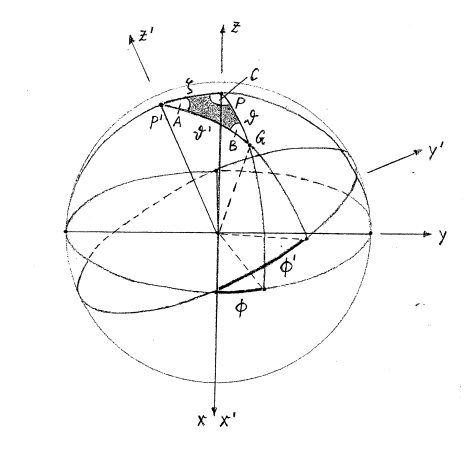
\includegraphics[width=0.6\linewidth]{./Trigonometrie}
  %\caption{}
  \label{fig:Trigonometrie}
\end{figure}


\begin{atiSubtasks}
\item Schreiben Sie die Transformationsformeln auf, die die Koordinaten $(x,y,z)$ bei Drehung um den Winkel $\zeta$ in die Koordinaten $(x',y',z')$ überführen.
\item Führen Sie anstelle der kartesischen Koordinaten $(x,y,z)$ die Kugelkoordinaten $(r,\vartheta,\phi)$ ein (mit $r=R;$ für die gestrichenenen Koordinaten entsprechend).
\item Ersetzen Sie die Azimute $\phi$ und $\phi'$ durch die Innenwinkel $C$ bzw. $A$ des sphärischen Dreiecks und gewinnen Sie so
\begin{itemize}
\item den sphärischen Sinussatz
\[
\sin\vartheta'\sin A=\sin \vartheta \sin C,
\]
\item sphärische Kosinus-Formel (manchmal auch Sinus-Kosinus-Satz) genannt
\[
\sin \vartheta'\cos A=-\sin \vartheta \cos C\cos \zeta+\cos \vartheta\sin \zeta
\]
\item den sphärischen Seiten-Kosinussatz
\[
\cos \vartheta'=\sin\vartheta \cos C\sin\zeta+\cos \vartheta\cos \zeta.
\]
\item In diesen Formeln treten die Winkel $A$ und $C$ zusammen mit den ihnen gegenüberliegenden Dreiecksseiten $\theta$ bzw. $\theta'$ auf. Leiten Sie die entsprechenden Resultate, in den der Winkel $B$ vorkommt, durch zyklische Vertauschung her.
\end{itemize}
\end{atiSubtasks}
\end{atiTask}
